\documentclass[a4paper,abstract=on,twoside,parskip=full]{scrreprt}
\setlength\parindent{1.5em}

\usepackage[todo]{../../common/naps62}

\hypersetup{pdfauthor={André Martins Pereira}}
\hypersetup{pdftitle={Pre-Thesis: Efficient processing of ATLAS events analysis in platforms with accelerating devices}}

\bibliography{../../common/bib/gpu}

% reduce chapter margins
\renewcommand{\chapterheadstartvskip}{\vspace*{-1.6\baselineskip}}

\begin{document}
\pdfbookmark{Cover}{cover}
\pagenumbering{roman}
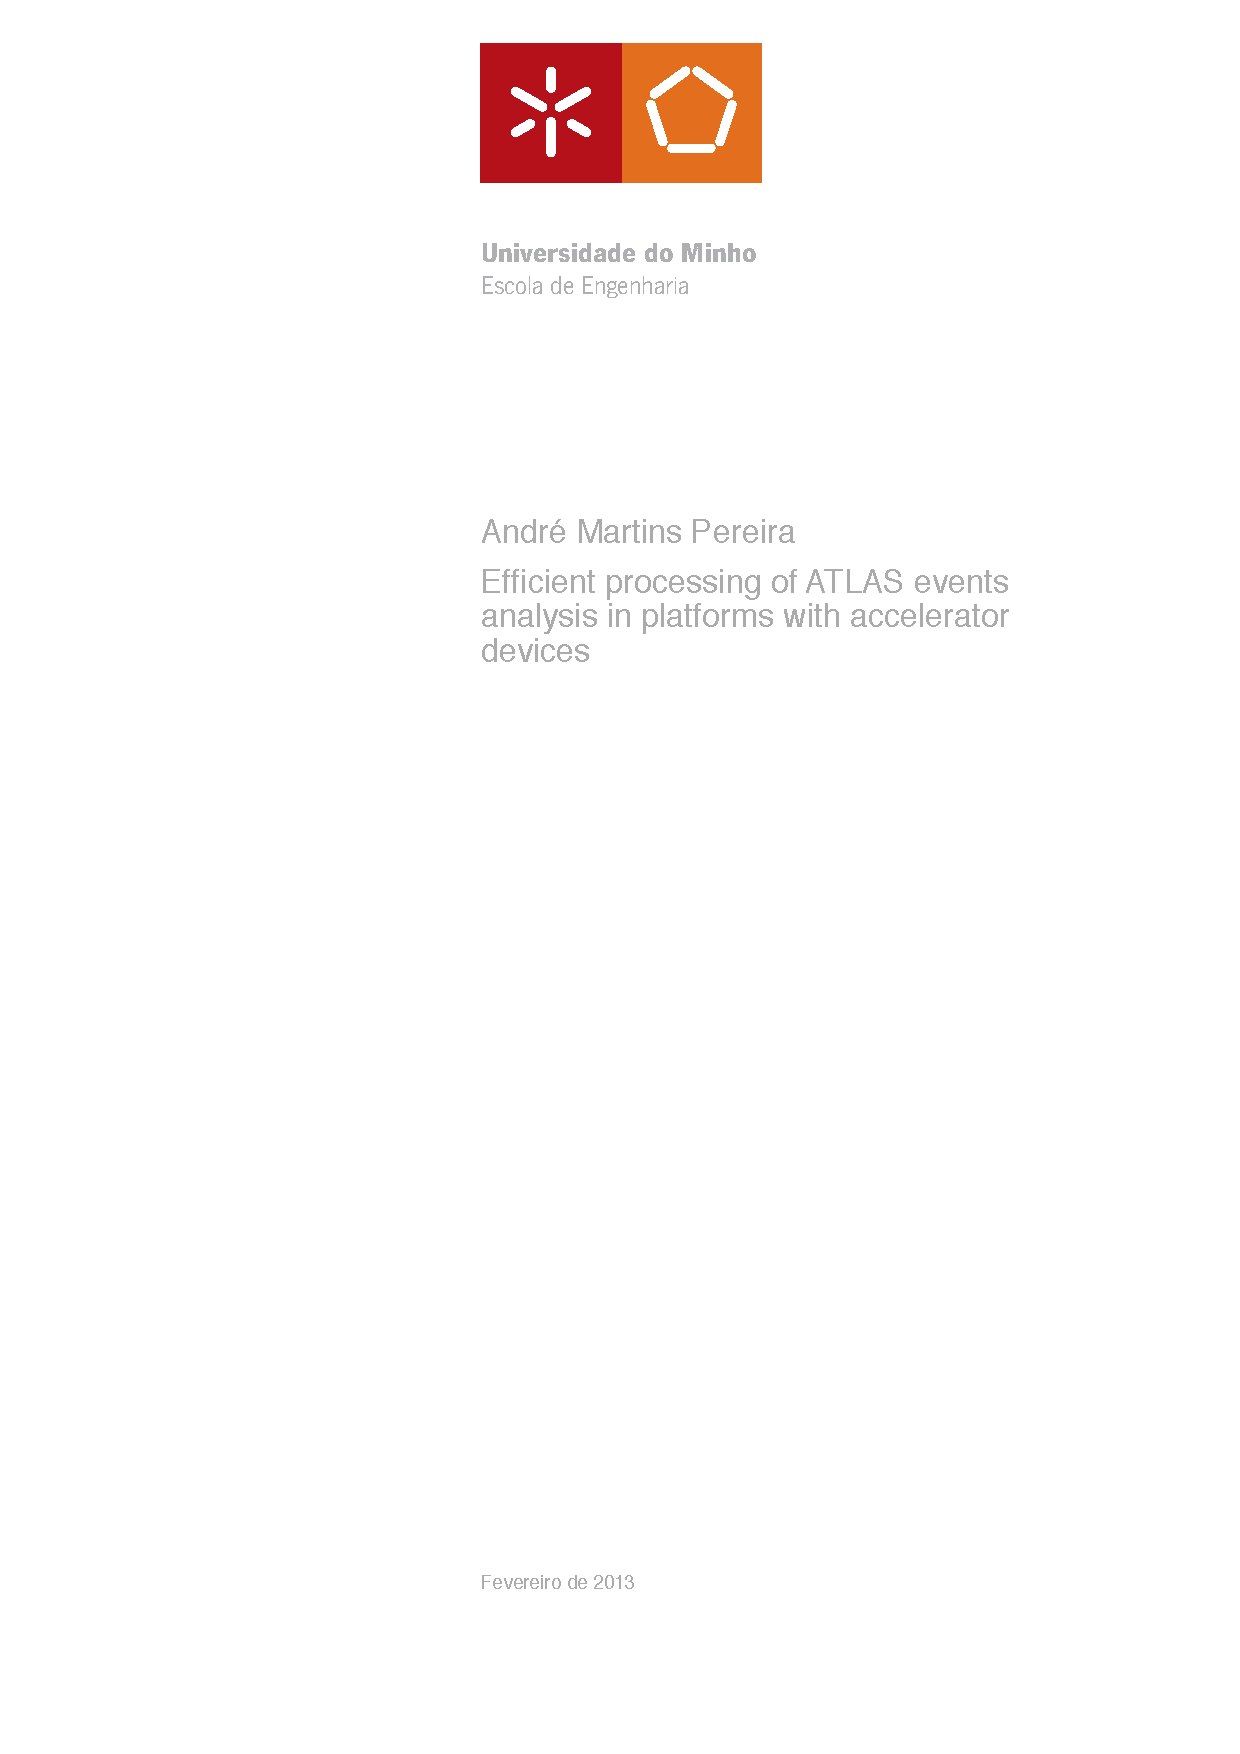
\includepdf[pages=-]{misc/cover-mei}

\pagestyle{fancy}
\renewcommand{\headrulewidth}{0.4pt}
\fancyhead[LO,RE]{}
\fancyhead[LE]{\slshape \leftmark}
\fancyhead[RO]{\slshape \rightmark}
\fancyfoot[RO,LE]{\thepage}%
\fancyfoot[C]{}

\fancypagestyle{plain}{%
  \renewcommand{\headrulewidth}{0.0pt}
  \fancyhead{}
  \fancyfoot[C]{}
  \fancyfoot[RO,LE]{\thepage}
}


%
% include all tex/ chapter files
%
%\bash[stdoutFile=/dev/null,stderrFile=/dev/null,exitCodeFile=/dev/null,scriptFile=bash.out]
%ls tex/ | egrep ^[^_] | sed "s/\([^.]*\)\.tex/\\\\subfile{tex\/\1}/" > tex/_inputs.tex
%\END

\pdfbookmark{Resumo}{resumo}
\chapter*{Resumo}

A maior parte das tarefas de análise de dados de eventos no projeto ATLAS requerem grandes capacidades de acesso a dados e processamento, em que q performance de algumas das tarefas são limitadas pela capacidade de I/O e outras pela capacidade de computação.

Esta dissertação irá focar-se principalmente nos problemas limitados computacionalmente nas últimas fases de análise dos dados do detector do ATLAS (as calibrações), complementando uma dissertação paralela que irá lidar com as tarefas limitadas pelo I/O.

O principal objectivo deste trabalho será desenhar, implementar, validar e avaliar uma tarefa de análise mais robusta e melhorada, que envolve aperfeiçoar a performance da reconstrução kinemática de eventos dentro da framework usada para a análise de dados no ATLAS, a ser executada em plataformas de computação heterogénea baseada em CPUs multicore acoplados com placas PCI-E com dispositivos many-core, tais como o \intel Xeon Phi e/ou os dispositivos GPU \nvidia Fermi/Kepler.

Uma aplicação de análise será usada como caso de estudo, desenvolvida pelo grupo LIP, para melhorar a reconstrução kinemática, bem como restruturar e paralelizar outras regiões críticas desta análise.

Uma framework experimental, GAMA, será usada para automatizar (i) a distribuição de carga pelos recursos disponíveis e (ii) a gestão transparente de dados através do ambiente de memória física distribuída, entre a memória partilhada do CPU multicore e da memória dos dispositivos many-core. Ela será comparada com outra framework similar, OpenACC, em termos de performance, tempo de desenvolvimento e usabilidade.

\newpage \pdfbookmark{Abstract}{abstract}
\chapter*{Abstract}

Most event data analysis tasks in the ATLAS project require both intensive data access and processing, where some tasks are typically I/O bound while others are compute bound.

This dissertation work will mainly focus on compute bound issues at the latest stages of the ATLAS detector data analysis (the calibrations), complementing a parallel dissertation work that addresses the I/O bound issues.

The main goal of the work is to design, implement, validate and evaluate an improved and more robust data analysis task which involves tuning the performance of the kinematical reconstruction of events within the framework used for data analysis in ATLAS, to run on computing heterogeneous platforms based on multi-core CPU devices coupled to PCI-E boards with many-core devices, such as the \intel Xeon Phi and/or the \nvidia Fermi/Kepler GPU devices.

As a case study, an analysis application will be used, developed by the LIP research group, to tune the kinematical reconstruction, as well as restructure and parallelize other critical areas of this analysis.

An experimental framework, GAMA, will be used to automate (i) the workload distribution among the available resources and (ii) the transparent data management across the physical distributed memory environment between the shared multi-core memory and the many-core device memory. It will be compared against a similar concurrent framework, OpenACC, in terms of performance, development time and usability.

\newpage
\pagenumbering{arabic}


\pdfbookmark{Contents}{contents}
\tableofcontents

\newpage \pdfbookmark{Glossary}{glossary}
\chapter*{Glossary}
\begin{acronym}
  \acro{Event}{Head-on collision between two particles at the LHC}
  \acro{Combination}{A set of two leptons and two jets}
  \acro{LHC}{Large Hardron Collider particle accelerator}
  \acro{ATLAS project}{Experiment being conducted at the LHC with an associated particle detector}
  \acro{LIP}{Laboratório de Instrumentação e Física Experimental de Partículas, Portuguese research group working in the ATLAS project}
  \acro{CERN}{European Organization for Nuclear Research, which results from a collaboration from many countries to test HEP theories}
  \acro{HEP}{High Energy Physics}
  \acro{Analysis}{Application developed to process the data gathered by the ATLAS detector and test a specific HEP theory}
  \acro{Accelerator device}{Specialized processing unit connected to the system by a PCI-Express interface}
  \acro{CPU}{Central Processing Unit, which may contain one or more cores (multicore)}
  \acro{GPU}{Graphics Processing Unit}
  \acro{GPGPU}{General Purpose Graphics Processing Unit, recent designation to  scientific computing oriented GPUs}
  \acro{DSP}{Digital Signal Processor}
  \acro{MIC}{Many Integrated Core, accelerator device architecture developed by \intel, also known as Xeon Phi}
  \acro{QPI}{Quickpath Interconnect, point-to-point interconnection developed by \intel}
  \acro{HT}{HyperTransport, point-to-point interconnection developed by the HyperTransport Consortium}
  \acro{NUMA}{Non-Uniform Memory Access, memory design where the access time depends on the location of the memory relative to a processor}
  \acro{ISE}{Instruction Set Extensions, extensions to the CPU instruction set, usually SIMD}
  \acro{Homogeneous system}{Classic computer system, which contain one or more similar multicore CPUs}
  \acro{Heterogeneous system}{Computer system, which contains a multicore CPU and one or more accelerator devices}
  \acro{SIMD}{Single Instruction Multiple Data, describes a parallel processing architecture where a single instruction is applied to a large set of data simultaneously}
  \acro{SIMT}{Single Instruction Multiple Threads, describes the processing architecture that \nvidia uses, very similar to SIMD, where a thread is responsable for a subset of the data to process}
  \acro{SM/SMX}{Streaming Multiprocessor, SIMT/SIMD processing unit available in \nvidia GPUs}
  \acro{Kernel}{Parallel portion of an application code designed to run on a CUDA capable GPU}
  \acro{Host}{CPU in a heterogeneous system, using the CUDA designation}
  \acro{CUDA}{Compute Unified Device Architecture, a parallel computing platform for GPUs}
  \acro{OpenMP}{Open Multi-Processing, an API for shared memory multiprocessing}
  \acro{OpenACC}{Open Accelerator, an API to offload code from a host CPU to an attached accelerator}
  \acro{GAMA}{GPU and Multicore Aware, an API for shared memory multiprocessing in platforms with a host CPU and an attached CUDA enabled accelerators}
  \acro{Speedup}{Ratio of the performance increase between two versions of the code. Usually comparing single vs multithreaded applications.}

  bottleneck
\end{acronym}

\newpage \pdfbookmark{List of Figures}{figures}
\listoffigures
\newpage

\chapter{Introduction}
\label{Introduction}

\begin{quote}
\textit{The dissertation is first presented by contextualizing the scientific background of CERN and LIP organizations, as well as their current research projects, which are closely involved in this work. The motivation for the dissertation is presented in section \ref{Motivation}, with the problem contextualized from a physics perspective in subsection \ref{TopQuarkSystem}. The Goals, subsection \ref{Goals}, states the objectives to be achieved by this work, in terms of improving the research and application development quality by implementing a set of solutions for homogeneous and heterogeneous systems, while assessing the efficiency and usability of hardware accelerators in the latter. The scientific contribution of this work is presented in subsection \ref{ScientificContribution}. Subsection \ref{DissertationStructure} overviews the structure of this dissertation.}
\end{quote}

\section{Context}
\label{Context}

The European Organization for Nuclear Research \cite{CERN} (CERN, acronym for \textit{Conseil Européen pour la Recherche Nucléaire}) is a consorcium of 20 european member countries with the purpose of operating the largest particle physics laboratory in the world. Founded in 1954, CERN is located in the border between France and Switzerland, and employs thousands of scientists and engineers representing 608 universities and research groups and 113 different nationalities.

CERN research focus on the basic constituents of matter, which started by studying the atomic nucleus but quickly moved into high energy physiscs (HEP), focusing on the interaction between particles. The instrumentation used in the nuclear research, physics-wise, is essentially divided into particle accelerators and detectors, alongside with the facilities necessary for delivering the protons to the accelerators. The purpose of the accelerator is to speed up groups of particles close to the speed of light, in opposite directions, and collide them in the detectors (this collision is called an event). The detectors record various characteristics, such as energy and momentum, of particles resultant from complex decay processes of the original particles. These experiments are performed to test and validate specific HEP theories by comparing the results of the collision to the expected theoretical model.

It started with a small low energy particle accelerator, the Proton Synchrotron \cite{CERN:PS} inaugurated in 1959, but the facilities were iteratively being upgraded and expanded. The current facilities are constituted by the older accelerators (some decomissioned while others are still functional) and detectors, as well as the newer Large Hadron Collider (LHC) \cite{CERN:LHC} high energy particle accelerator which is located 100 meter underground and has a 27 km circuference length. There are currently seven experiments running on the LHC: CMS \cite{CERN:CMS}, ATLAS \cite{CERN:ATLAS}, LHCb \cite{CERN:LHCb}, MoEDAL \cite{CERN:MoEDAL}, TOTEM \cite{CERN:TOTEM}, LHC-forward \cite{CERN:LHCf} and ALICE \cite{CERN:ALICE}. Each of these experiments has their own detector on the LHC and conduct similar or different experiments, but with the use of distinct technologies and research approaches. Currently one of the most popular researches being conducted is the validation of the Higgs boson theory. During the next year the LHC will be upgraded to increase its luminosity (amount of energy of the particle beams that it accelerates).
\todo{Fonte disto do upgrade}

Approximately 600 millions of collisions occur every second in each of the experiment's detectors at the LHC, where the detectors react to the particle interaction and produce electric signals, generating massive amounts of raw data. It's estimated that all the detectors combined produce 25 petabytes of data per year \cite{CERN:DATA1,CERN:DATA2}. CERN does not have the financial resources to have the computational power to process all the data, which motivated the creation of the Worldwide LHC Computing Grid \cite{CERN:WLHCCG}, a distributed computing infrastructure that uses the resources of scientific community for data processing. The grid is organized in a hierarchy divided in 4 tiers. Each tier is made by one or more computing centers and has a set of specific tasks and services to perform, such as store, filter, refine and analyse all the data gathered at the LHC.

The Tier-0 is the data center located at CERN. It provides 20\% of the total grid computing capacity, and its objective is to store and reconstruct the raw data gathered at the detectors in the LHC into meaningful information, usable by the remaining tiers. The data is received on a format designed for this reconstruction, with information about detector and software diagnostics. After the reconstruction the data has a different formats, the Event Summary Data (ESD) and Analysis Object Data (AOD), each one with different purposes, containing information of the reconstructed objects and calibration parameters, and can be used for early analysis. This tier distributes the raw data and the reconstructed output by the 11 Tier-1 computational centers, spread among the different countries that are members of CERN.

Tier-1 computational centers are responsible for storing a portion of the raw and reconstructed data and provide support to the grid 24/7. In this tier, the reconstructed data suffers more reprocessing, in order to refine it by filtering only relevante information and reducing the size of the data, now in Derived Physics Data (DPD) format, that is then transferred to the Tier-2 computational centers. The size of the data for an event is reduced from ~3 MB (raw) to ~10 kB (DPD). This tier also stores the outputs of the simulations performed at Tier-2. The Tier-0 center is connected to the 11 Tier-1 centers by high bandwidth optical fiber links, which consists of the LHC Optical Private Network.

There are around 140 Tier-2 computational centers around the world. Their main purpose is to perform Monte-Carlo simulations with the data received from the Tier-1 centers, but also perform a portion of the events reconstructions. The Tier-3 centers range from university clusters to small personnal computers, and they perform most of the events reconstruction and final data analysis. In the CERN related groups terminology, an analysis is a denomination for an application which is designed to process a given amount of data in order to test a specific HEP theory by providing physically relevant information about events that may support the said theory.

\section{LIP Research Group}
\label{LIP}

The Laboratório de Instrumentação e Física Experimental de Partículas (LIP) \cite{LIP} is a portuguese scientific and technical association for research on experimental high energy physics and associated instrumentation. LIP has a strong collaboration with CERN as it was the first scientific organization Portugal has joined, in 1986. It has laboratories in Lisbon, Coimbra and Minho and 170 people employed. LIP researchers have produced several applications for testing various HEP theories of the ATLAS experiment that use Tier-3 computational resources for data analysis. Most of the analysis applications use home-grown frameworks, such as the LipCbrAnalysis and LipMiniAnalysis.

This dissertation work results from a close cooperation between the Department of Informatics of the University of Minho and the LIP laboratory in Minho.

\todo{Falar aqui do que se trata o trabalho ou referir que está explicado mais a frente?}

\section{Motivation, Goals \& Scientific Contribution}
\label{Motivation}

With an increase of events and, consequently, the data being produced by the detectors at the LHC, specifically in the ATLAS experiment, the research groups will need a bigger budget for aquiring and maintaining computational resources due to an increase of analysis to perform. To add up to this data increase, research groups working on the same experiment have a positive rivalry to be the first find and publish relevant results. The finding of these results is directly related to the amount of events processed, meaning that groups with more computational resources are one step ahead.

Better results are not only obtained by increasing the amount of events analyzed; it is important to take into account the quality of each analysis. The ATLAS detector has an experimental resolution of 2\%, meaning that each measured value for a characteristic of a resultant particle of a collision might not be real and, therefore, the analysis will have an error associated. It is possible to improve the analysis quality but it will increase its execution time, creating a trade-off between events to analyze and their quality. This issue will be presented in the context of this dissertation with more detail on subsection \ref{TopQuarkSystem}.

One of the most important analysis being conducted by LIP is related to the Top Quark physics and the Higgs Boson. An application was devised that reconstructs an event following the theoretical model of Top Quark decay and then also attempts to reconstruct the associated Higgs Boson. Each event can be reconstructed several times, with some of its parameters slightly varied by a random offset (with a maximum magnitude of 2\% of the original value), and by chosing the reconstruction that satisfies the most the theoretical model a better solution is obtained, overcoming the experimental resolution of the ATLAS detector. The more reconstructions per event are performed the longer will take to process an event. The theoretical model for this system is presented in subsection \ref{TopQuarkSystem} and the analysis application in chapter \ref{Application}.

While investing in the upgrade of the computational resources of the research group is a valid option to deal with the increase of events to analyze, it is also necessary to take into account if the current resources are being efficiently used by the analysis applications. Also, hardware is not necessarily getting faster, but wider by increasing the number of cores per chip (see chapter \ref{TechnologicalBackground}), which can cause big investments to result in small improvements. Current computing clusters are constituted of systems with one or more multicore CPUs (homogeneous systems) and some even utilizing hardware accelerators, very efficient for specific problem domains (heterogeneous systems). It is important to have a knowledge of these newer architectures in order to develop efficient applications that resort to parallelism in order to better use all the resources available in a system. Programming for such architectures (multicore CPUs and hardware accelerators) requires a set of skills and experience that most physicists (usually self-taught programmers) do not have, causing poorly optimized applications to be developed.

Increasing the efficiency of an application by resorting to parallelism enables the possibility of performing more reconstructions per event and more events to be processed, while using all the potential of the available computational resources and avoiding needless investments in hardware upgrades.

\subsection{The Top Quark system and Higgs boson decay}
\label{TopQuarkSystem}

In the LHC two proton beams are accelerated close to the speed of light in opposite directions, set to collide inside a specific particle detector. From this head-on collision results a chain reaction of decaying particles, from which only some of the final particles react with the detector for recording their characteristics. One of the experiments being conducted at the ATLAS detector is related to the discovery of new Top Quark physics. The schematic representation of the Top Quark decay (the \ttbar system), resulting from a head-on collision of two protons, is presented in figure \ref{fig:TopQuarkDecay}.

\begin{figure}[!htp]
	\begin{center}
		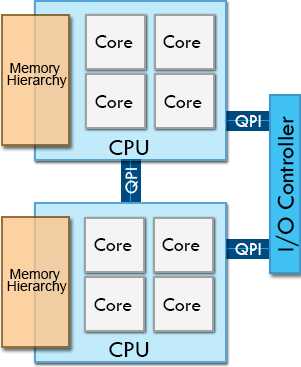
\includegraphics[scale=0.5]{../../common/img/numa_qpi.png}
		\caption{Schematic representation of the \ttbar system.}
		\label{fig:TopQuarkDecay}
	\end{center}
\end{figure}

The ATLAS detector is able to record the characteristics of Bottom Quarks, which are detected as a jet rather than a single particle, and leptons, the muon (that has a positive charge) and electron (with a negative charge). However, the neutrinos do not react with the detector and, therefore, their characteristics are not recorded. To reconstruct the Top Quarks, necessary for researching their properties, it is necessary to have the information of all the final particles, so the neutrino characteristics must be determined. This is possible to do as the \ttbar system obeys a set of properties, and using the information of the quarks and leptons the neutrinos characteristics are analitically calculated. The process of reconstructing the neutrinos is referred as kinematical reconstruction. The reconstruction of the whole \ttbar system has a degree of certainty associated, which determines its quality. The quality of these reconstructions directly affects the quality of the research being conducted by LIP.

The amount of Bottom Quark jets and leptons detected may vary between events, due to other reactions occurring at the same time of the Top Quark decay. As represented in figure \ref{fig:TopQuarkDecay}, it is needed 2 jets and 2 leptons to reconstruct the \ttbar system, but the data for an event may have many of these particles associated. To obtain the best reconstruction for the \ttbar system of a given event it is necessary to reconstruct the respective neutrinos and then the whole system for every combination of 2 jets and 2 leptons, and only chose the most accurate reconstruction.

Another factor affecting the quality of the reconstruction is the experimental resolution of the ATLAS particle detector, which associates an error of 2\% with every measurement made. If the measurements of the jets and leptons are not precise enough the kinematical reconstruction will produce inaccurate neutrinos and affect the overall reconstruction of an event, which might render an event with relevant physics useless. It is possible to overcome this problem by performing the kinematical reconstruction, and then the whole \ttbar system reconstruction, a large amount of times for each combination of 2 Bottom Quark jets with 2 leptons, with a random variation to the particle characteristics (momentum, energy and mass) of a maximum magnitude of 2\% of the original value. The amount of variations performed per combination will directly impact the final quality of the event reconstruction, as more of the search space (defined by the experimental resolution error) is covered compared to performing a single reconstruction. The more variations are performed the more likely it is to find the best possible reconstruction of the \ttbar system.

The look for the Higgs Boson is also part of the research being conducted at LIP. Figure \ref{fig:HiggsBosonDecay} schematizes the Higgs Boson and Top Quark decay. It is possible to reconstruct the Higgs Boson from the two Bottom Quark jets that it decays to, and it can be performed alongside the \ttbar system reconstruction. This adds at least two more jets to the event information, and it is not possible to know before the reconstruction which jets belong to the Higgs decay or the Top Quark decay. Considering this, the Higgs reconstruction must be performed after the \ttbar system reconstruction, in such a way that the jets chosen to reconstruct it must not be the ones used in the \ttbar system reconstruction. Adding this new jets increases the number of jets/leptons combinations to test in the kinematical reconstruction, and for each \ttbar system reconstruction the Higgs must be also reconstructed. Now, the quality of the event reconstruction depends on the quality of both \ttbar system and Higgs Boson reconstructions.

\begin{figure}[!htp]
	\begin{center}
		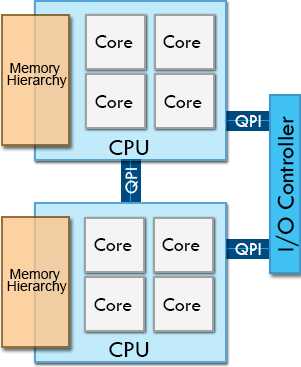
\includegraphics[scale=0.5]{../../common/img/numa_qpi.png}
		\caption{Schematic representation of the \ttbar system with the Higgs Boson decay.}
		\label{fig:HiggsBosonDecay}
	\end{center}
\end{figure}

This specific analysis of events presented is performed by an application developed by LIP researchers, the \tth. The application receives input data file with a set of events and reconstructs the \ttbar system and the Higgs Boson for each event using the processes described. These files are usually 1 GB long and the LIP research requires that hundreds of them are processed by the same application, considering a specific experiment such as the presented in this subsection. A in-depth computational analysis of \tth is presented in chapter \ref{Application}, where its flow is presented, it is characterized in terms of various metrics (such as computational intensity) and the critical regions are identified.

\subsection{Goals}
\label{Goals}

By increasing the performance of the Top Quark and Higgs Boson reconstructions it is possible to perform more variations per event, increasing the quality of the results, and increase the throughput of events processed. The objective of this dissertation work is to take a sequential application made by physicists, which the main concern during its development was the correcteness of the code rather than its performance, the \tth, and improve its efficiency by (i) identifying the bottlenecks and optimizing the code, (ii) increasing the performance by resorting to parallelism for homogeneous and heterogeneous systems, assessing the efficiency (performance and usability) of hardware accelerators for this type of problem, and (iii) the development of a simple scheduler for managing the workload among various instances of the same sequential or parallel application (i.e. an application which needs to process a large set of separate input files) on homogeneous systems.

This work will give a inside perspective of how scientific applications are being developed by programmers with little to no background in computer science, and possibly define a set guidelines for coding of efficient applications and the usage of parallelism in such applications. All the changes that will be made to the \tth application, including the introduction of parallelism, will be as independent as possible from the context of this specific problem, in such a way that they might be portable to other applications without requiring major modifications. The work will be structured, implementation wise, so that the parallelization mechanisms and the scheduler are possible to be improved and transformed in a tool used by the researchers at LIP.

\subsection{Scientific Contribution}
\label{ScientificContribution}

This dissertation work aims to improve the quality of a specific research field conducted by LIP, provide a set of tools and know-how to improve the performance of similar scientific applications and expose the problematic of unefficient usage of computational resources. By improving the quality of the research, LIP will gain an advantage over other research groups in the look for new Top Quark physics and in the Higgs Boson discovery. By experiencing the process of optimizating scientific applications of this kind it is possible to provide physicists with some know-how and tools for optimization and parallelization with the goal of increasing the performance in future applications. By developing applications that efficiently use all the computational resources available it is possible to reduce the investment in new hardware, which otherwise would have small pratical returns.

\section{Dissertation Structure}
\label{DissertationStructure}

This dissertation has 5 chapters and their summary is presented below:

\begin{description}
	\item[Introduction] \hfill \\
	The dissertation is first presented by contextualizing the scientific background of CERN and LIP organizations, as well as their current research projects, which are closely involved in this work. The motivation for the dissertation is presented in section \ref{Motivation}, with the problem contextualized from a physics perspective in subsection \ref{TopQuarkSystem}. The Goals, subsection \ref{Goals}, states the objectives to be achieved by this work, in terms of improving the research and application development quality by implementing a set of solutions for homogeneous and heterogeneous systems, while assessing the efficiency and usability of hardware accelerators in the latter. The scientific contribution of this work is presented in subsection \ref{ScientificContribution}. Subsection \ref{DissertationStructure} overviews the structure of this dissertation.
	\item[Technological Background] \hfill \\
	This chapter presents the current technological state of the art in terms hardware and software. Hardware-wise, both homogeneous and heterogeneous system architectures and details are presented in sections \ref{HomogeneousSystems} and \ref{HeterogeneousSystems}, respectively. A contextualization of current hardware accelerators is also made in the latter. Software-wise is presented in section \ref{Software}. Various frameworks and libraries are presented for homogeneous systems and accelerators in sections \ref{pThreads}, \ref{OpenMP}, \ref{MPI} and \ref{CUDA}. Section \ref{HeterogeneousFrameworks} presents the available frameworks for parallelization in heterogeneous systems. Finally, current solutions for profiling and debugging parallel applications is presented in section \ref{ProfilingDebugging}.
	\item[\tth Application] \hfill \\
	The \tth application for event reconstruction is presented in this chapter. Its dependencies are presented. The flow of the application is presented in section \ref{Application:Flow}, accompanied by a schematic representation. Its main functions are presented and the schematic flow is compared against a callgraph of the application to help understanding what happens in each of the most important functions. The critical region is identified in section \ref{CriticalRegion} and characterized in subsection \ref{ComputationalCharactrization}. Some initial optimizations to the code are presented in subsection \ref{InitialOptimizations}.
	\item[Parallelization Approaches] \hfill \\
	For different parallelization alternatives are presented in this chapter. For homogeneous systems, a shared memory parallelization is discussed in section \ref{Parallelization:SharedMem}, where the abstract heuristic used is shown, and the implementation and a performance analysis are presented in subsections \ref{SharedMemImplementation} and \ref{SharedMemPerformance}, respectively. For heterogeneous systems using hardware accelerators, two alternatives are presented: using GPU as an accelerator, in section \ref{Parallelization:GPU}, with its implementation and performance discussed and analyzed in subsections \ref{GPUImplementation} and \ref{GPUPerformance}; using the \intel Xeon Phi as an accelerator in section \ref{Parallelization:MIC} and its implementation discussed in subsection \ref{MICImplementation}. A software scheduler for managing workload distribution among applications for homogeneous shared memory systems is presented in section \ref{Parallelization:Scheduler}. Its implementation details and performance analysis are shown in subsections \ref{SchedulerImplementation} and \ref{SchedulerPerformance}.
	\item[Conclusions \& Future Work] \hfill \\
	This chapter concludes the dissertation, presenting an overview of the results obtained by the work developed, on both homogeneous and heterogeneous systems. Guidelines for future work, on improving the test case application and providing parallel solutions abstracted from the programmer for future application development, are presented.
\end{description}


\chapter{Contextualization}
\label{context}

The LHC accelerates two particle beams in opposite directions, causing them to collide at the particle detectors. From this head-on collision between two particles results a limited chain reaction of decaying particles, where the detector records the characteristics of most of the final particles. A schematic representation of the head-on collision, and respective particle decay, is presented in figure \ref{fig:ttbar}, and it is known as the \ttbar system. The detected particles are the bottom quarks (which are detected as a jet of particles) and leptons (electron and muon), while the neutrinos do not react with the detector and, therefore, are not detected. To reconstruct the collision, the characteristics of these neutrinos must be determined. Since this system obeys a set of properties, related to the calibrated model expected from the collision, it is possible to analytically determine the neutrinos characteristics and reconstruct the event (kinematical reconstruction), and then estimate the degree of certainty associated with the computed reconstruction.

\begin{figure}[!htp]
	\begin{center}
		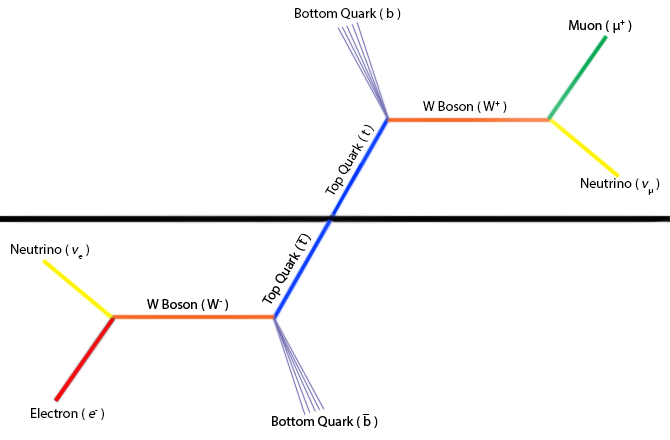
\includegraphics[scale=0.5]{../../common/img/ttbar.png}
		\caption{Schematic representation of the \ttbar system.}
		\label{fig:ttbar}
	\end{center}
\end{figure}

The amount of bottom quark jets and leptons detected can vary between events. However, it is needed at least 2 jets and 2 leptons are needed to reconstruct the \ttbar system, as represented in the figure~\ref{fig:ttbar}, but their amount can reach up to 14. Some of the jets/leptons may not belong to the \ttbar system (as other reactions occur during the collision), so there is a need to choose the ones that most accurately reconstruct the system. Note that the quality of the reconstruction has a strong impact the quality of the research being conducted by the LIP group.

By performing the kinematical reconstruction to each combination of all the bottom quark jets and leptons, two by two, and computing the probability associated with the respective reconstruction, it is possible to chose only the combination that results on the most accurate reconstruction.

Another factor that can affect the accuracy of the reconstruction is the experimental resolution associated with the ATLAS detector. The detected values for the particles (bottom quark jets and leptons) are not fully accurate: the measurements made by ATLAS can have a 2\% fluctuation to the real values. Since these particles are used in the kinematical reconstruction, its accuracy can be impaired. To improve the quality of these reconstructions, the experimental resolution must be compensated. This can be achieved by varying the values of the bottom quark jets and leptons characteristics, such as the mass or momentum, and use them in the kinematical reconstruction. However, this cannot be performed only once: the search space must be covered a certain amount of times to get higher probability of finding a great reconstruction. This means running the kinematical reconstruction as many times as possible, per event, with different variations of the original inputs (jet/lepton combination).

The execution time of the analysis is critical due to the large amounts of data (events) that must be processed. Since for each event it is necessary to reconstruct all the bottom quark jets and leptons combinations, and for each combination a variation is applied several times, the number of kinematical reconstructions per event can quickly rise, increasing the overall time to process an event. A must be achieved balance between the required quality of the reconstruction, directly related to the number of times that the kinematical reconstruction is performed, and the time that takes to process an event. 

The relevance of the kinematical reconstruction (dilep) is even greater in the \tth analysis. This analysis aims to reconstruct the Higgs boson based on the two jets that decay from it. Figure \ref{fig:ttbarhiggs} schematically represents the \ttbar system with the Higgs boson decay and respective jets. However, the jets that decay from the Higgs boson cannot be differentiated from the other similar jets. After performing the \ttbar system reconstruction, i.e., the kinematical reconstruction, and considering the jets used in its best reconstruction, the application uses the remaining jets to reconstruct the Higgs boson. If an event \ttbar system is not properly reconstructed, the Higgs boson reconstruction will not be accurate. The best final reconstruction is the one with the higher combined probabilities of the best kinematical reconstruction and the respective best Higgs boson reconstruction. 

\begin{figure}[!htp]
	\begin{center}
		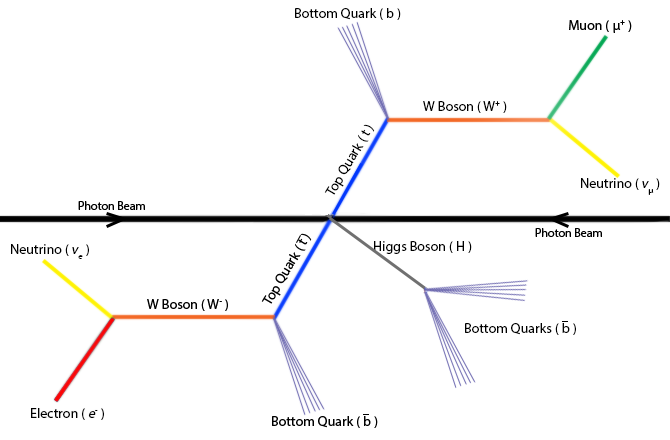
\includegraphics[scale=0.5]{../../common/img/ttbar_higgs.png}
		\caption{Schematic representation of the \ttbar system with the Higgs boson decay.}
		\label{fig:ttbarhiggs}
	\end{center}
\end{figure}

By increasing the performance of the kinematical reconstruction it is possible to compute more reconstructions per event, leading to better and more accurate results. However, it is not possible to narrow the scope of this dissertation work only to the reconstruction; to get the most efficiency from it, it is necessary to consider other tasks to improve, such as the jet combination, variance appliance and Higgs reconstruction, and eventually re-design the workflow of this section of the application. The LIP research group needs to improve the performance of both kinematical reconstruction and the overall \tth analysis, to improve the overall results quality of the ATLAS project, giving them an advantage over the other teams.

\newpage


\chapter{State of the Art}
\label{stateart}

Most of today’s programmers produce code and design applications using sequential programming paradigms. The application behavior is designed and tested only for sequential execution, where the only parallelism is made by the compiler at the instruction level. A few years ago a transition from single core very fast CPUs to slightly slower multicore CPUs started to happen. Unfortunately, these newer CPUs need a different programming paradigm to get the most performance possible when designing an application; programmers did not accompany this transition to parallel programming paradigms.

Programming for multicore environments require some knowledge of the underlying architectural concepts. Shared memory, cache coherence and consistency and data races are architectural aspects that the programmer did not have to face in sequential execution environments. Now, when designing an application, all these aspects must be taken into account, not only to ensure efficient use of the computational resources, but also the correctness of the application.

Heterogeneous computer architectures are becoming increasingly popular. They combine the flexibility of multicore CPUs with the specific capabilities of many-core accelerator devices, connected by PCI-Express interfaces. However, most computational algorithms and applications are designed with the specific characteristics of CPUs in mind. Even multithreaded applications cannot be easily ported to these devices expecting high performance. To optimize the code for these specific devices it is necessary to deeply understand the architectural principles behind their design.

These devices are usually made from small processing units, designed to achieve the most performance possible on specific problem domains, as opposed to common \"all-around\" CPUs. They are oriented for massive data parallelism processing (SIMD architectures), offloading the CPU from such data intensive operations. Several many-core accelerator devices are available, ranging from the general purpose GPUs, to the \intel Many Integrated Core line, currently known as \intel Xeon Phi \cite{Intel:MIC}, and Digital Signal Processors (DSP) \cite{Texas:DSP}. A heterogeneous platform may have one or more accelerator devices of the same or different types.

Many libraries and frameworks were already developed for these new heterogeneous platforms. They range from frameworks to abstract the inherent complexity of these systems, such as OpenACC \cite{OpenACC} or GAMA \cite{GAMA}, to specialized high performance libraries for some specific scientific domains, such as CuBLAS \cite{NVIDIA:CuBLAS}.

A more in-depth analysis of these two groups of state of the art technology (hardware and software) will be presented through the next sections.

\section{Hardware}

While having the same (conceptual) purpose, different accelerator devices opt to use different approaches to solve their domain specific problems, leading to small, but important, architectural differences. If these details are not taken into account, it is impossible to make efficient code, underusing the specialized resources of these devices.

The Single Instruction Multiple Data (SIMD) parallelism model is common ground for most accelerator devices architectures. It is designed to get the most throughput when processing information by applying the same instruction, in parallel, to large sets of independent data. Considering the GPUs and image processing as an example, each pixel that is rendered is independent from all other pixels on the image. Their computation result from the same instructions but on different independent data, thus making their processing embarrassingly parallel. For achieving maximum performance, one important characteristic of the code, common to most accelerator device architectures, is that it needs to explore the most parallelism possible between the data to be processed. Other device specific properties, with interest for the programmer, will be discussed later.

Load balancing is always a challenge when programming for parallel environments. Even when using only multicore CPUs, it is important to manage how much load each core is processing, so that every core is working most of the time. If the workload is badly distributed, there will be cores stalled waiting for others to complete, wasting the available computatuinal resources. However, it also depends on the nature of the problem; regular problems are easier to balance than irregular problems, which usually require a dynamic load balancing strategy at runtime, since the execution time of the parallel tasks is not predictable.

Heterogeneous architectures open the possibility of running parallel tasks on both CPU and accelerators simultaneously. However, due to their technical differences, the same task can take different amount of time to complete depending in where it is executed. This creates another layer of complexity when dealing with the workload balance. Now, while managing the workload distribution inside the CPU (between its cores), and also inside the accelerator device chip (with a mechanism similar to the CPU), it is also relevant to manage the distribution between CPU and accelerator device. It is important to have a good control over the load balancing, specially in these hybrid systems, in such a way that neither of the processing units (CPU and accelerator devices) becomes stalled waiting for the other to complete, and thus not wasting any computational resources. Also, the load balancing must be done with the least communication possible between CPU and accelerator, since the time it takes to complete is usually high.

\subsection{Graphics Processing Unit}

There are several accelerator devices currently arriving, or already, on the market. The first and most common are General Purpose Graphics Processing Units (GPGPUs). Recently, GPGPU makers allowed drivers to execute code that is not produced for image rendering. However, there are specific hardware details that were designed only for image rendering purposes, which limit the utilization of these devices for certain types of algorithms. One example was the use of only single precision float point arithmetic in the early GPGPUs design.

As mentioned before, this type of devices are specialized for massive data parallelism, where the same instruction is applied to large amounts of data simultaneously. One example of a problem domain that can take advantage of these characteristics is the multiplication of matrices, which is very common in scientific applications. As GPGPUs evolved, the support for specific scientific demands was added, such as support for double precision float point arithmetic and compliance to all IEEE float point arithmetic rules.

Recently, \nvidia \cite{NVIDIA} launched a line of GPUs designed for scientific computation rather than image processing \cite{NVIDIA:Tesla}. This category of devices, known as the Tesla, has more GDDR ram, processing units and a slight different design suitable for use in cluster computational nodes (in terms of size and cooling). The chip has suffered some changes too, increasing the cache and the amount of processing units. In this dissertation two different \nvidia GPUs will be used, the \nvidia Tesla C2070 (Fermi architecture \cite{NVIDIA:Fermi}) and the new \nvidia Tesla based on the \textbf{GK110} chip (Kepler architecture \cite{NVIDIA:Kepler}).

\nvidia GPUs architecture has two main components: computing units (Streaming Multiprocessors, known as SM) and memory  (global memory, GDDR5 ram, and cache inside the SM). Each SM contains a set of \cuda cores, which are processing units that perform both integer and float point arithmetic (additions, multiplications and divisions). These SMs also have some specialized processing units for only square roots, sins and cosines, as well as a warp scheduler (warps will be explained later) to match \cuda threads to \cuda cores, load and store units, register files and a 2 level cache hierarchy.

\nvidia considers that a parallel task is constituted by a set of \cuda threads, which will execute the same instructions (conditional jumps are a special case that will be explained next) but on different data. This set of instructions is considered a \cuda kernel, in which the programmer defines the behavior of the \cuda threads. A simple way to visualize this concept is by considering the example of multiplying a scalar with a matrix. In this case, a single thread will handle the multiplication of the scalar by an element of the matrix, and it is needed to use as many \cuda threads as matrix elements.

The \cuda threads are organized in a hierarchy. A block is a set of \cuda threads that is matched by the global scheduler to run on a specific SM. A grid is a set of blocks, representing the whole parallel task. Considering the scalar-matrix multiplication example, each \cuda thread calculates the value of an element of the matrix, and they are organized in blocks, which can represent all the calculations for a single line of the matrix. The grid holds all the blocks responsible for calculating all the new values of the matrix. Note that both the block and the grid have a limited size.

A warp is a set of \cuda threads (usually the same amount as the number of the \cuda cores available in a SM), scheduled by the SM scheduler to run on its SM at a given time. A warp can only be constituted by \cuda threads from the same block.

When programming for these devices, conditional jumps must be avoided at all costs. Within an SM it is not possible to have 2 threads executing different instructions at the same time. So, if there is a divergence between the threads within the same warp, the two conditional branches will be executed one after the other, doubling the warp execution time.

Since the GPU is connected by PCI-Express interface, the bandwidth for communications between CPU and GPU is restricted to only 12 GB/s (6 GB in each direction of the communication). Memory transfers between the CPU and GPU must be minimal as it greatly restricts the performance.

Architecture specific details, relevant to the programmer, of both Fermi and Kepler will be presented in the next subsections.

\subsubsection{\nvidia Fermi Architecture}

The relevant architectural details of this architecture, specifically for the Tesla C2070, are explained in this section. The Fermi architecture is schematized in figure \ref{fig:fermi}.

\begin{figure}[!htp]
	\begin{center}
		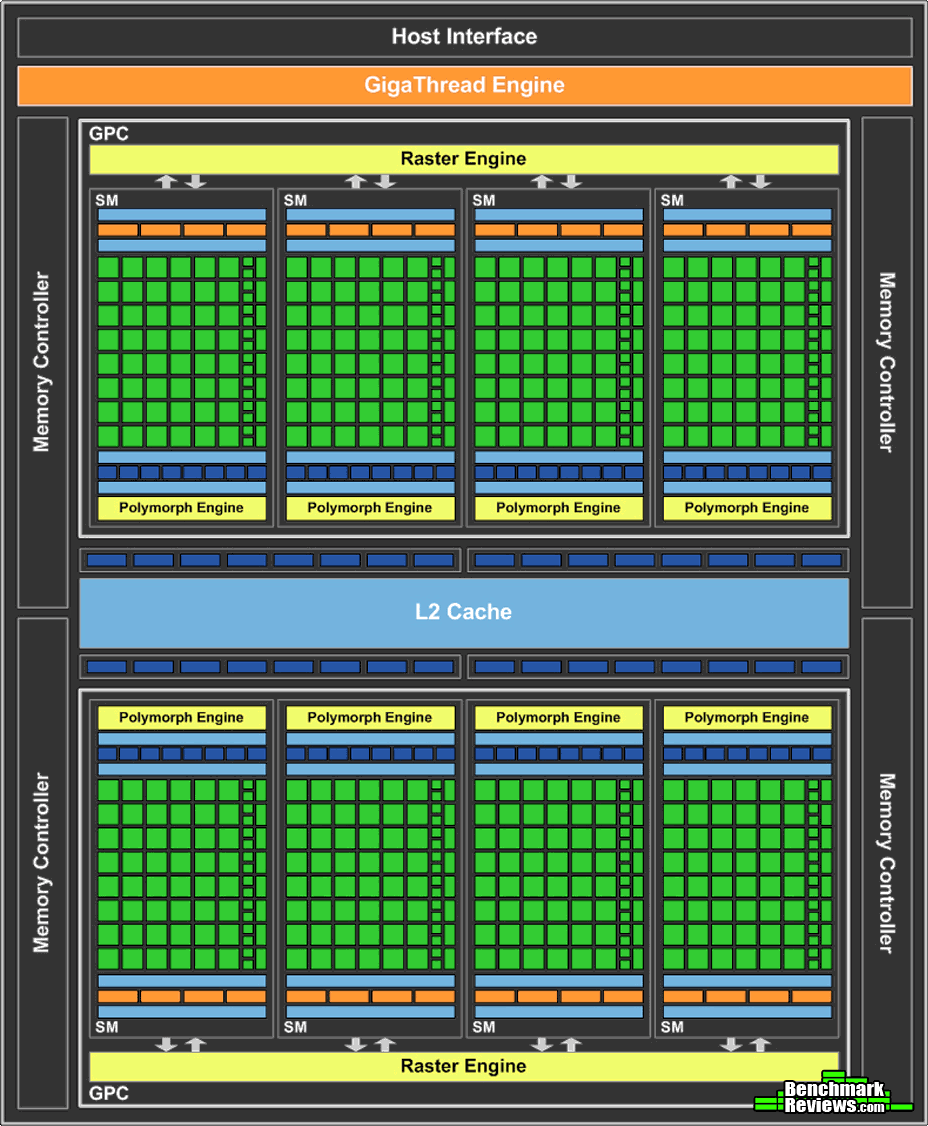
\includegraphics[scale=0.25]{../../common/img/fermi_arch.png}
		\caption{Schematic representation of the \nvidia Fermi architecure.}
		\label{fig:fermi}
	\end{center}
\end{figure}

In the Tesla C2070, each SM has 32 \cuda cores, with 14 SM per chip, making a total of 448 \cuda cores. Theoretically, it is possible to have 448 \cuda threads running at the same time. In each SM there is 4 Special Functional Units (SFU) to process square roots, sins and cosines.

Memory wise, these devices have a slightly different memory hierarchy than the CPUs, but still with the faster and smaller memory is closer to the \cuda cores. Each \cuda thread can have up to 63 registers, but when large amounts of threads are used this amount diminishes, which can, in some cases, lead to register spilling (when there is not enough registers to hold the variables values and they must be stored in the cache).

Within a SM there is a block of configurable 64 KB memory. In this architecture it is possible to use it as 16 KB for L1 cache and 48 KB for shared memory (only shared between threads of the same block) or vice versa. The best configuration is dependent of the specific characteristics of each algorithm, and usually requires some preliminary tests to evaluate which configuration obtains the best performance. Shared memory can also be used to hold common resources to the threads, even if they are read only, avoiding accesses to the slower global memory.

The L2 cache is slower but larger, with the size of 768 KB. It is shared among the SMs, opposed to the L1 cache. The global memory is the last level of on device memory. The Tesla C2070 has a total of 6 GB GDDR5 ram, with a bandwidth of 192.4 GB/s.

One important detail for efficient memory usage is to perform coalesced memory accesses. Since the load units get memory in blocks of 128 bits, it is possible to reduce the amount of loads by guaranteeing that all the threads that need to load data, preferably if it is continuous on the address space (such as elements of an array), do it at the same time. This allows the memory controller to find the best grouping of thread loads and consolidates them in the fewer memory accesses possible \cite{NVIDIA:Fermi}.

Finally, on the Fermi architecture it is only possible to run one kernel at a time on the GPU.

\subsubsection{\nvidia Kepler Architecture}

The Kepler and Fermi architectures have many similarities so only the relevant differentiating aspects will be presented.

The Streaming Multiprocessor present in the Fermi architecture was changed to hold more, but smaller, \cuda cores (now 192), working at half the speed of the previous \cuda cores, and it is now known as SMX. This allows having up to 2880 \cuda cores in only one chip, which can be seen in the representation of the Kepler architecture in figure \ref{fig:kepler}.

The maximum amount of registers per \cuda thread was increased from 63 to 255. A new read-only cache of 48 KB was added at the same hierarchy level of the L1 cache. The size of the L1/shared memory block is the same as Fermi, but adds a new configuration of 32/32 KB for each type. The L2 cache size has increased to 1536 KB, and its hit bandwidth is 73\% larger than on Fermi.

\begin{figure}[!htp]
	\begin{center}
		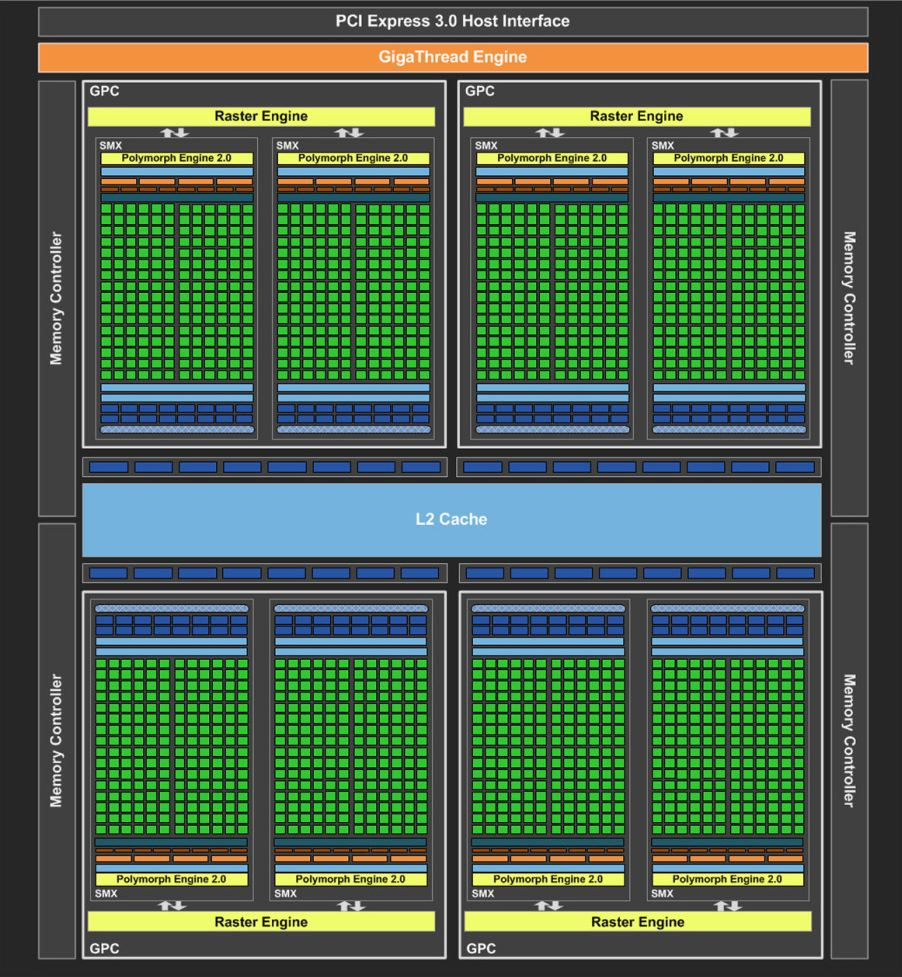
\includegraphics[scale=0.4]{../../common/img/kepler_arch.jpg}
		\caption{Schematic representation of the \nvidia Kepler architecture.}
		\label{fig:kepler}
	\end{center}
\end{figure}

Programming-wise, a set of new important features has been added to this architecture. One of them is the Dynamic Parallelism. Now it is possible to \cuda threads spawn other threads, without it being explicitly required by the host (CPU). It allows for improvements in irregular problems, such as Monte Carlo ray tracing. Another feature is the Hyper-Q, which allows multiple cores of the same CPU to use and spawn kernels on the same GPU. Also, it is now possible to run several different kernels in the same GPU at the same time, where they will be scheduled to different SMX. Finally, a new shuffle instruction has been added to the instruction set. By using this instruction \cuda threads can now read values directly from each other, within the same warp, without the need of using shared memory.

The problem of coalesced memory accesses is still present. However, while Fermi load units get blocks of 128 bits, load units on the Kepler architecture are capable of getting blocks of 256 bits \cite{NVIDIA:Kepler}.

\subsection{\intel Many Integrated Core}

The \intel Many Integrated Core (MIC), currently known as \intel Xeon Phi, architecture from Intel, Knights Corner, has a different conceptual design than the Nvidia GPUs. A chip can have up to 61 multithread cores, with 4 threads per core, and it is more focused on vectorization \cite{Intel:MIC:Elgar}. 

\begin{figure}[!htp]
	\begin{center}
		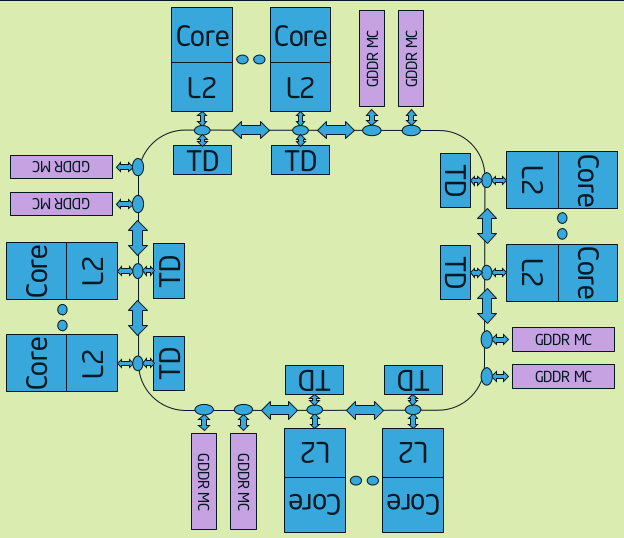
\includegraphics[scale=0.5]{../../common/img/mic_arch.png}
		\caption{Schematic representation of the \intel MIC architecture.}
		\label{fig:mic}
	\end{center}
\end{figure}

It has 32 512 bit wide vector registers per core, with the capacity of holding 16 single precision float point values. The L2 cache size is 512 KB per core and the chip comes with 6 to 8 GB of GDDR5 ram, providing up to 320 GB/s of throughput. It was designed for memory bound problems, as oposed to GPUs (Fermi only has a bandwidth of 192.4 GB/s), but Intel will also launch a different version of the chip tuned for compute bound problems.

Unlike CPUs, the MIC cores do not share any cache, therefore cache consistency and coherence is not assured. If needed, data must be explicitly passed between cores, as in a distributed memory system. The cores are connected in a ring network, as represented in figure \ref{fig:mic}.

The MIC uses the same instruction set as common \intel CPUs (x86). This allows to easily port current libraries to run on this device. Furthermore, Intel has already announced that a tuned MPI library will be available for this device.

\section{Software}

Application development for homogeneous systems with multicore CPUs is not as recent as one may think. There are some libraries that attempt to abstract the programmer from specific architectural and implementation details, providing an easy API as close as possible to current sequential programming paradigms.

However, developing applications for heterogeneous systems, with both CPU and accelerator devices, poses a series of new challenges due to the change of programming paradigm. Even though, there are some frameworks that attempt to abstract the inherent complexity of these platforms.

Frameworks that attempt to ease the programmer’s job, while providing scalable and flexible solutions, which will be used during the dissertation, will be presented through the next subsections. Other frameworks that will not be used, such as Threading Building Blocks from \intel \cite{Intel:TBB}, will not be discussed.

\subsection{OpenMP}

For shared memory systems, where there is one or more multicore CPUs sharing the same memory address space, one of the most popular libraries for task parallelization is OpenMP \cite{OpenMP}. This API is designed for multi-platform shared memory parallel programming in C, C++ and Fortran, on all available CPU architectures. It is portable and scalable, aiming to provide a simple and flexible interface for developing parallel applications, even for the most inexperienced programmers.

While being simple to use, OpenMP allows experienced users to fine-tune the code, providing various task schedulers, as well as instructions for controlling more efficiently the shared memory accesses and parallel execution of the tasks.

\subsection{OpenACC}

OpenACC \cite{OpenACC} is a framework for heterogeneous platforms with accelerator devices. It is designed to simplify the programing paradigm for CPU/GPU systems by abstracting the memory management, kernel creation and GPU management. Like OpenMP, it is designed for C, C++ and Fortran, but allowing the parallel task to run on both CPU and GPU at the same time.

While it was originally designed only for CPU/GPU systems, they are currently working on the support for the new Intel Xeon Phi \cite{OpenACC:HPCWire}. Also, they are working alongside with the members of OpenMP to create a new specification supporting accelerator devices in future OpenMP releases \cite{OpenACC:OpenMP}.

\subsection{GAMA}

The GAMA framework \cite{GAMA} with the same purpose as OpenACC but opts for a different strategy. It aims to create an abstraction layer between the architectural details of heterogeneous platforms and the programmer, aiding the development of portable and scalable parallel applications. However, unlike OpenACC, its main focus is on obtaining the best performance possible, rather than abstracting the architecture from the programmer. As consequence, there is more work for the programmer to develop an application, as, for example, it is necessary to define the dicing method (which will be used by GAMA to distribute the dataset). It is also possible to code the kernel that is to run in each device and other specific details.

Even though, the framework frees the programmer from managing the workload distribution, memory usage and data transfers between the available resources. Again, the programmer can have total control over these details.

This framework is capble of abstracting the address space of the heterogeneous platform (CPU and the accelerator device memory) used as a shared memory system. One particularity of this tool is that, even though it is capable of handling shared memory systems with one or more multicore CPUs, it is only capable of handling \cuda capable GPUs as accelerator devices on the system.

\subsection{Debugging}

Debugging applications in shared memory systems is a complex task, as the errors are usually harder to replicate than on sequential applications. Bugs can happen due to deadlocks, unexpected changes to the shared memory, data inconsistency and incoherence. While there are some tools to efficiently debug sequential applications, such as the GNU Debugger \cite{GDB}, they lack on the support for multithreaded applications. Unfortunately, there are no debuggers that can efficiently be used to debug a parallel application.

The effort necessary to debug these applications, without the use of any third-party tools, is directly related to the programmers experience and knowledge of working with shared memory systems. However, even the most experienced will face complex obstacles when debugging for more than 4 threads, as the application behavior is much harder to control.

Nvidia offers a tool for debugging \cuda kernels on their GPUs, which is based on the GNU Debugger \cite{NVIDIA:gdb}. It is useful when used to find bugs in the kernels, but only in the same way that a sequential application is debugged. Also, when using more than 2-4 \cuda threads it does not help the programmer at all, considering that \cuda kernels can reach to the thousands of threads.

\newpage


\chapter{Case study: the ttH\_dilep analysis application}

The computing resources related to all CERN projects are organized in a tier hierarchy. The first is the CERN Tier-0 computing clusters and from there is distributed to the 10 Tier-1 data centers, spread by different countries, which are used for central processing and reconstruction of data events and simulation of Monte Carlo events. Tier-2 sites are dedicated to further processing and reconstruction of data and Monte Carlo events, while Tier-3 sites are used to perform data analysis and simulation \cite{LIP:Ibergrid}.

\begin{figure}[!htp]
	\begin{center}
		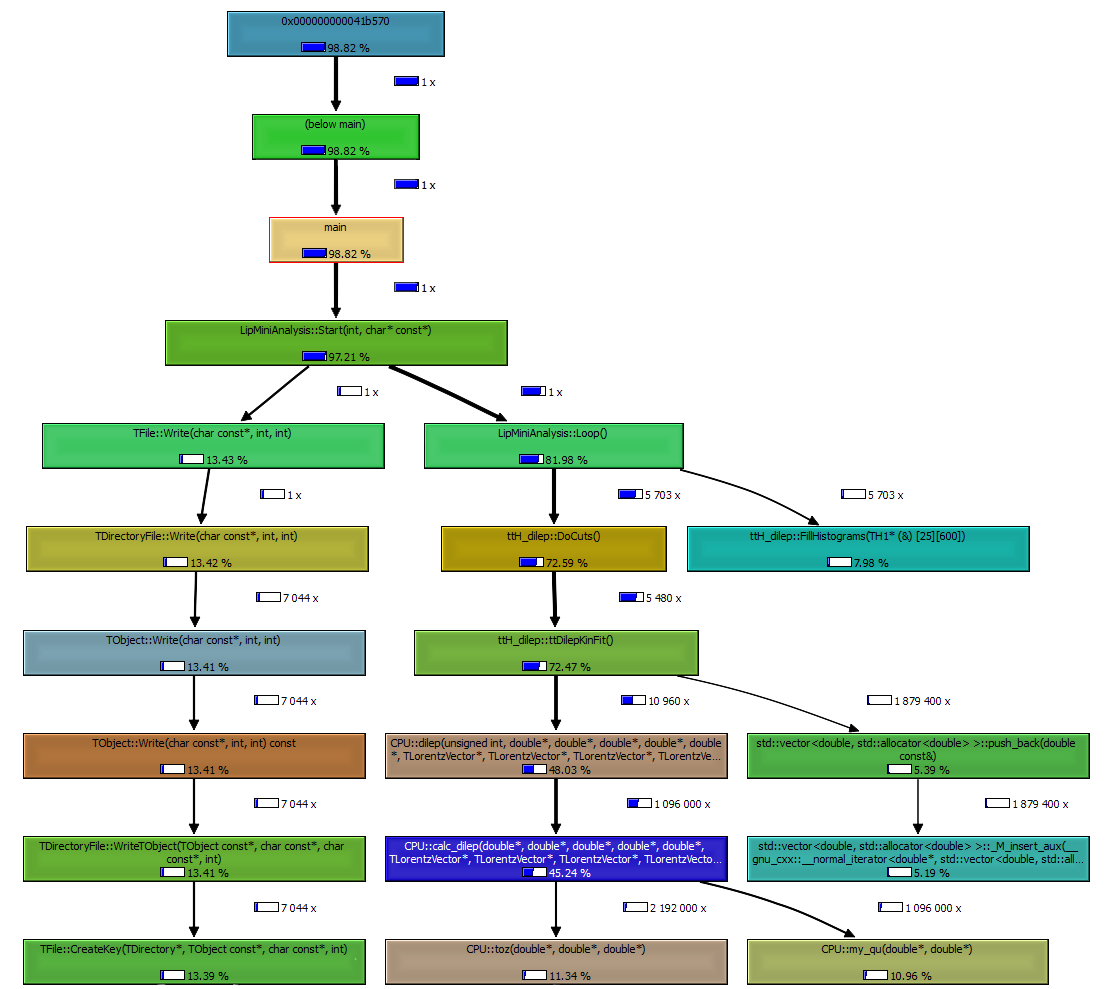
\includegraphics[scale=0.6]{../../common/img/callgraph_O3_100dilep.png}
		\caption{Callgraph generated using the Valgrind tool \cite{Callgrind} for the ttH\_dilep analysis with 100 dilep executions per event.}
		\label{fig:callgraph}
	\end{center}
\end{figure}

It is in this Tier-3 that the ttH\_dilep analysis application fits. It was developed by the LIP researchers to solve the problem explained in the section 2. The application has two main dependencies: the ROOT framework \cite{CERN:ROOT} and the LipMiniAnalysis library.

The ROOT framework is being developed by CERN and provides a set of functionalities needed to handle and analyze large amounts of data. They range from data storage, in the standard formats used by CERN, to histograming, curve fitting minimization and visualization methods. It aims to provide the programmer a set of tools that will ease the construction of their analysis code.

The LipMiniAnalysis is a library developed by LIP, containing a set of methods and functionalities useful for the analysis that they conduct with the ATLAS detector data. It is also prepared to read a more refined set of data resultant from the DPD data format that arrives at the Tier-3.

As illustrated by the callgraph of the analysis application in figure \ref{fig:callgraph}, the main flow of the application is controlled by the Loop method. This method will apply the DoCuts function to every event to process. The event passes a series of tests and evaluations (cuts). If an event reaches the cut 20, of a total of 21, the ttDilepKinFit function is called. It is in this function that the ttbar and Higgs reconstructions are performed. In the beginning of the ttDilepKinFit method, the available jets are combined two by two, as well as the leptons, as explained in section 2.

The dilep function, called after within the ttDilepKinFit method, analytically determines the neutrinos characteristics for each jets and leptons combination, reconstructing the ttbar system. It can produce two to four possible result particles. These results are used in the remaining of the ttDilepKinFit to determine the probability of the reconstruction, as well as reconstruct the Higgs boson. The final probability of the reconstruction is determined by combining the probability of the ttbar reconstruction with the calculated probability of the Higgs reconstruction.
As seen from the callgraph, most of the application execution time is spent in the Loop method, so there is the place where most efforts of optimization must be focused. The rest are auxiliary and I/O functions.

\newpage


\chapter{Conclusions and Future Work}

The workflow of the ttDilepKinFit method, explained in the previous section, needs to be changed so that it can be easier and more effective to parallelize its execution. Currently, the variation is applied for each jet/lepton combination, dilep is executed, the results are treated (and the probability of the reconstruction is calculated) and the Higgs boson is reconstructed.

The best approach is to create a data set with all the jet/lepton combinations and all the respective amount of variations. Then, execute dilep with all the elements on the data set and store all the results with the associated element of the data set. Note that the number of dilep executions per event will be equal to the number of jet/lepton combination times the number of variations per combination.  Finally, iterate through all of the results, reconstruct each Higgs boson and calculate the respective probability for each element of the first data set. Figure \ref{fig:pipeline} represents the current and the presented alternative workflows.

\begin{figure}[!htp]
	\begin{center}
		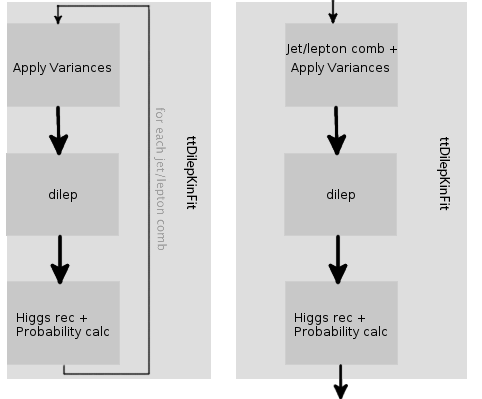
\includegraphics[scale=0.5]{../../common/img/pipeline.png}
		\caption{Current workflow (left) vs alternative workflow (right) of the ttDilepKinFit method.}
		\label{fig:pipeline}
	\end{center}
\end{figure}

This approach offers (theoretically) the possibility of having three distinct parallel tasks. The first would be the jet/lepton combination and variance calculations. The second, would be the dilep executions, which are independent, it is only needed to merge the results after. The third would be the final iteration through the results of each dilep execution and respective Higgs reconstruction. However, these three parallel tasks are dependent on each other. 

To ease the cost of this dependency a queue-based approach will be tested. As the first data set is constructed, its elements can be provided to the next parallel task, where dilep is executed. As soon as the results from dilep are available they can be passed to the third parallel region and the Higgs boson can be reconstructed. In theory, this will decrease the execution time, relative to a strict implementation, where all the parallel tasks are being executed at the same time after an initial latency. Figure Z1 illustrates the current workflow of ttDilepKinFit and the alterations that will be made.

After this stage, an implementation of the kinematical reconstruction (dilep), which is the most time consuming task in the Loop method, and it tends to increase even more with the number of variances specified, will be attempted on both GPUs and Xeon Phi. The efforts will be towards obtaining the most optimal hybrid (i.e., also using the CPU) implementation possible. The performance will be measured and compared between these devices and the bottlenecks identified.

Finally, an implementation using the OpenACC and GAMA frameworks will be tested, relatively to the previous optimized implementations, in terms of performance but also considering the development time and usability of these tools.

\newpage



%\bibliographystyle{../../common/IEEE}
%\nocite{*}
\newpage % force the bookmark to go to the new page
\pdfbookmark{References}{references}
\printbibliography[title=References]

\end{document}
